\RequirePackage{fix-cm}
\documentclass[twocolumn]{svjour3}
\smartqed
\usepackage{graphicx}
\tolerance=1
\emergencystretch=\maxdimen
\hyphenpenalty=10000
\hbadness=10000
\def\makeheadbox{\relax}
\usepackage[numbers]{natbib}
\usepackage{multirow}%
\usepackage{amsmath,amssymb,amsfonts}%
\usepackage{mathrsfs}%
\usepackage[title]{appendix}%
\usepackage{textcomp}%
\usepackage{manyfoot}%
\usepackage{booktabs}%
\usepackage{algorithm}%
\usepackage{algorithmicx}%
\usepackage{algpseudocode}%
\usepackage{listings}%

%%% Additional packages from original manuscript
\usepackage{tabularx}
\usepackage{url}
\usepackage{tikz}
\usetikzlibrary{arrows.meta, positioning, shapes.geometric}
\usepackage[dvipsnames,table]{xcolor}

\usepackage{enumitem}
\usepackage{pgfplots}
\pgfplotsset{compat=1.12}
\usepackage{float}
\usepackage{stfloats}

\renewcommand{\algorithmicrequire}{\textbf{Input:}}
\renewcommand{\algorithmicensure}{\textbf{Output:}}


\begin{document}


\title{An Empirical Study of Kubernetes HPA Behavior for Stateful WebSocket Workloads}

\titlerunning{HPA Behavior Under Stateful WebSocket Workloads}

\author{
Abhash Behera \and
Aditya Hota \and
Suprit Kumar Naik \and
Ritesh Kumar Singh \and
Rakesh Ranjan Kumar\thanks{Corresponding author. Email: rakeshranjan@cgu-odisha.ac.in} \and
Binita Kumari
}

\authorrunning{Behera et al.}
\institute{
Department of Computer Science and Engineering,\\
C V Raman Global University,\\
Bhubaneswar 752054, Odisha, India\\
\\
Emails:\\
2301020213@cgu-odisha.ac.in,\\
2301020486@cgu-odisha.ac.in,\\
2301020457@cgu-odisha.ac.in,\\
2301020845@cgu-odisha.ac.in,\\
rakeshranjan@cgu-odisha.ac.in,\\
binita.kumari@cgu-odisha.ac.in
}

\date{}

\maketitle

\begin{abstract}
Kubernetes' Horizontal Pod Autoscaler (HPA) scales deployments using a
proportional control law built around CPU utilization. That works fine for
stateless, request-driven services, but it runs into trouble with stateful,
persistent-connection protocols such as WebSocket, where session state lives on a
specific pod whether or not the connection happens to be busy at that moment. Kill
the pod and every connection it was holding goes with it. We ran four controlled
experiments to pin down exactly how this plays out. Experiment~A gives us a
correct-behavior baseline under near-ideal conditions. Experiment~B1 puts HPA
through a realistic HIGH/LOW activity cycle and shows it over-provisions badly and
recovers slowly. Experiment~B2-Instrumented measures what actually happens during a
scale-down event: a large reconnection storm that hits right as pods are terminated
and throws the session population into disarray. Experiment~B3 then shows that when
clients don't retry on their own, these events destroy sessions permanently, in a
staircase pattern, with nothing bringing the numbers back. Across all four
experiments, the failure traces back to how HPA's CPU-based design interacts with
persistent-connection workloads rather than to any single misconfigured parameter.
CPU simply isn't a good stand-in for connection demand, and tuning parameters alone
doesn't fix it. These findings feed directly into the connection-aware autoscaling
approach explored in subsequent work.
\end{abstract}

\keywords{Kubernetes \and Horizontal Pod Autoscaler \and WebSocket \and Stateful Workloads \and Autoscaling \and Reconnection Storm \and Cloud Computing \and Performance Evaluations}


%% ============================================================
\section{Introduction}
\label{sec:intro}
%% ============================================================

Kubernetes has become the default choice for container orchestration in the
cloud~\cite{hightower2017kubernetes,merkel2014docker}, and a big part of why people
like it is the Horizontal Pod Autoscaler (HPA), which watches resource metrics on a
fixed cycle and adjusts replica counts through a proportional control
law~\cite{k8s_hpa_docs,nguyen2020hpa,burns2016borg}. For ordinary HTTP services,
where CPU load tracks request volume reasonably well, this works about as expected
~\cite{casalicchio2017auto,lorido2014auto}.

The problem shows up with WebSocket~\cite{websocket_rfc} and similar protocols: a
connection that stays open for minutes, sometimes hours, doing full-duplex work the
whole time. Persistent WebSocket connections, MQTT, collaborative editors,
multiplayer games, IoT gateways, and long-lived streaming pipelines are all
increasingly common in production, so getting autoscaling right for them actually
matters. For these workloads, CPU isn't really the resource that counts -
what counts is the open connection itself, since the session state sits on one
particular pod. Terminate that pod and every connection it held drops at the same
instant, so every affected client tries to reconnect at once. We call this a
reconnection storm.

Here's the core issue in one sentence: CPU usage tells you nothing about
how many connections a pod is actually holding. A pod can be quietly serving 800
healthy WebSocket sessions while barely touching the CPU, and from HPA's point of
view that looks identical to a pod doing nothing at all - so it gets removed
either way.

None of this is a brand-new observation. Dickel et al.~\cite{dickel2019evaluation}
already pointed out that stateful protocols don't play well with HPA. What's
missing from that prior work is any real measurement of how bad the problem gets, or
a concrete reconnection-storm rate. That's the gap we're trying to close here, and
our contributions break down as follows:

\begin{enumerate}[leftmargin=*]
\item \textbf{Four experiments that build on each other.} A, B1, B2-Instrumented,
  and B3 run in sequence, moving from over-provisioning, to a measured reconnection
  storm, to permanent connection loss.

\item \textbf{An actual measured storm rate.} With Prometheus instrumentation in
  place, we measure a mean peak of 457~connections/second triggered by one single HPA
  scale-down decision. Earlier work only described this qualitatively; we put a
  number on it.

\item \textbf{A step-by-step account of the mechanism.} Experiment~B3 walks
  through the sequence: connections go idle, CPU drops toward zero, HPA scales
  down in response, and the sessions on the terminated pod are gone for good. All of
  this happens using nothing more exotic than default CPU-based HPA behavior.

\item \textbf{The stabilization window doesn't save you.} HPA's stabilization
  window smooths out CPU-derived replica recommendations - it has nothing to do
  with connection counts. Once CPU sits near zero for long enough, every value
  going into that window is \texttt{minReplicas}, so no matter how you size the
  window, the buffered output still ends up at \texttt{minReplicas}.

\item \textbf{Concrete numbers to benchmark against.} Every failure mode we
  describe comes with a number attached - 233\% replica over-allocation, a 457~conn/s
  storm peak, 18.8\% mean connection loss - which should give future autoscaling
  work something to compare against.
\end{enumerate}

As far as we can tell, this is one of the first empirical studies to systematically
characterize Kubernetes HPA behavior under persistent WebSocket workloads in a way
that actually quantifies reconnection storms, over-provisioning, and permanent
session destruction, all within one unified experimental setup.

The rest of the paper goes like this. Section~\ref{sec:related} covers related
work, Section~\ref{sec:background} gives a quick recap of the HPA control loop,
Section~\ref{sec:problem} walks through the four experiments in detail,
Section~\ref{sec:discussion} gets into why this happens and what it means in
practice, Section~\ref{sec:limitations} covers what we couldn't test, and
Section~\ref{sec:conclusion} wraps things up.



%% ============================================================
\section{Related Work}
\label{sec:related}
%% ============================================================

\subsection{Kubernetes HPA Architecture and Behavior}

Nguyen et al.~\cite{nguyen2020hpa} analyzed the HPA feedback loop and scrape
intervals, but their work assumes stateless HTTP services throughout; we instead
look at what happens under persistent WebSocket workloads, where CPU utilization
stops reflecting actual service demand. Recent studies characterizing Kubernetes resource management and autoscaling behavior similarly highlight the complexity of these operations~\cite{medel2024characterising}. Casalicchio
~\cite{casalicchio2019performance} showed that choosing relative versus absolute metrics
changes scaling stability, but again, their findings sit entirely within
HTTP/CPU workloads and don't touch connection-holding protocols. Lorido-Botr{\'a}n
et al.~\cite{lorido2014auto} lay out theoretical foundations
for proportional controllers and cloud resource adaptation more broadly; we lean on
that framing to show where these controllers actually break down for stateful
sessions.

\subsection{Custom and Application-Level Metrics for HPA}

Kubernetes does support custom metrics through the Prometheus
Adapter~\cite{prometheus_adapter}, but the existing literature mostly skips over
connection state entirely. Qu et al.~\cite{qu2018auto} and Rossi et
al.~\cite{rossi2019horizontal} propose enhanced autoscaling mechanisms, but they remain primarily focused on improving scaling efficiency rather than preserving persistent connection state. More recent predictive autoscaling schemes also rely on workload forecasting to improve HPA responsiveness~\cite{liu2023prediction}, but they continue assuming workload intensity is adequately represented through aggregate resource metrics. Recent industrial deployments such as AHPA~\cite{zhou2024ahpa} further improve scaling responsiveness using prediction models, but continue optimizing resource allocation rather than preserving application-level connection state. Our study targets exactly the
persistent-session problem these approaches miss, and we show that even with a
correct connection-count metric, HPA's stabilization window still buffers
metric-derived recommendations instead of connection-derived ones. That's a
structural limitation we dig into in Section~\ref{sec:discussion}.

\subsection{Stateful Workloads and Protocol-Aware Autoscaling}

Dickel et al.~\cite{dickel2019evaluation} flagged stateful autoscaling as an open
problem for WebSocket/MQTT gateways and suggested tracking active connections
through Prometheus, but they didn't validate this quantitatively. We take that
further and empirically characterize the actual failure modes, putting numbers on
the operational consequences these architectural gaps produce, which gives future
protocol-aware autoscaling work a baseline to work from.

\subsection{Graceful Connection Draining}

Production environments generally lean on \texttt{preStop} hooks and
\texttt{terminationGracePeriodSeconds}~\cite{k8s_container_lifecycle_hooks} so
stateless pods can drain in-flight requests before shutting down. That mechanism
just doesn't work for persistent sessions. A typical HTTP request resolves in
milliseconds; a WebSocket session can run for hours, so a standard grace period is
essentially irrelevant at that timescale. Experiment~B3 (Section~\ref{sec:b3})
puts a number on exactly how much permanent connection loss results when these
standard mechanisms fail to help.

\subsection{Research Gap}

Most existing studies evaluate HPA using stateless, request-driven workloads, or
they propose custom metrics without ever quantifying what CPU-driven scaling
actually costs under persistent connection workloads. Because of that, the
magnitude, reproducibility, and root cause of these failures remain poorly
characterized. This paper tries to close that gap by pinning down the exact
failure mechanisms with connection-second precision. Unlike Smart HPA~\cite{ahmad2024smarthpa}, which improves scaling decisions, our work empirically characterizes the inherent limitations of CPU-based HPA under persistent WebSocket workloads. Recent reinforcement learning approaches further improve Kubernetes autoscaling decisions using adaptive policies, but still optimize QoS and resource efficiency rather than preserving persistent connection state~\cite{khaleq2023intelligent}.



%% ============================================================
\section{Background: HPA Control Architecture}
\label{sec:background}
%% ============================================================

Before getting into the experiments, it helps to recap how the HPA control loop
actually works. Nguyen et al.~\cite{nguyen2020hpa} cover this in detail for
stateless workloads, and our own preliminary baselines reproduced their findings (Experiment A) -
staircase scale-up, CPU overshoot right as a burst starts, and negligible benefit
from scrape intervals below 30 seconds. That gave us confidence HPA behaves as
expected in the stateless case before we moved on to the stateful one. Feedback
control theory~\cite{hellerstein2004feedback} is the formal basis for the
proportional controller HPA implements, and elasticity in cloud computing is
defined formally in~\cite{herbst2013elasticity}.

\begin{figure*}[htbp]
\centering

\includegraphics[width=0.7\textwidth]{figures/K8-hpa-architecuture.png}
\caption{Overview of the Kubernetes Horizontal Pod Autoscaler (HPA) control architecture used throughout this study.}
\label{fig:hpa_arch}
\end{figure*}

Figure~\ref{fig:hpa_arch} shows the Kubernetes HPA control architecture we build on
throughout this paper. The controller runs the following discrete-time
proportional control law every 15~seconds, which is the default synchronization
period:
\begin{equation}
\textit{desiredReplicas} = \left\lceil \textit{currentReplicas} \times
  \frac{\textit{currentMetricValue}}{\textit{targetMetricValue}} \right\rceil
\label{eq:hpa}
\end{equation}

This formula assumes \texttt{currentMetricValue} actually reflects how busy the
workload is across every running replica. While production architectures often extend this mechanism using the Custom Metrics API and Prometheus Adapter, large-scale production Kubernetes deployments (e.g., CERN CMSWEB) similarly rely on extended observability and operational tooling around native Kubernetes autoscaling mechanisms~\cite{tedeschi2021cmsweb, ali2024cmsweb}. For CPU-based scaling of stateless
workloads that assumption mostly holds up. It falls apart for persistent-connection
workloads: an idle connection barely touches the CPU, yet it still represents a
committed piece of session state, and disrupting it is very visible to whoever is
on the other end. So the real experimental question is this: \textbf{what happens
when the control design's core assumption - that the signal tracks demand - is
simply not true?}



%% ============================================================
\section{Empirical Evidence of HPA Failure for Stateful WebSocket Workloads}
\label{sec:problem}
%% ============================================================

We ran a set of controlled experiments, each building on the last, designed to
isolate one failure mode of CPU-based HPA at a time when it's applied to
persistent WebSocket workloads. They're ordered from least severe
(over-provisioning) to most severe (permanent connection destruction), and each one
reuses the instrumentation and findings from the experiment before it.

All the WebSocket experiments share the same infrastructure and configuration,
summarized in Table~\ref{tab:architecture}. Everything runs on a 3-node Kind
cluster~\cite{kind_docs,merkel2014docker}, with the Metrics
Server~\cite{k8s_metrics_server} tuned for high-resolution scraping. The workload
itself is a custom Python asyncio WebSocket server we call \texttt{ws-instrumented}.
All the scripts, cluster configs, server code, and load generators used here are
public.

\begin{table}[!ht]
\centering
\caption{Summary of Experimental Architecture and Configuration}
\label{tab:architecture}
\begin{tabular}{ll}
\toprule
\textbf{Component} & \textbf{Configuration} \\
\midrule
Kubernetes & v1.31.6 \\
Kind & v0.25 \\
Worker nodes & 2 \\
Metrics Server & 15~s resolution \\
HPA target & CPU 60\% \\
Prometheus scrape interval & 15~s \\
WebSocket clients & 800 \\
\bottomrule
\end{tabular}
\end{table}

\paragraph{Instrumented server.}
By ``instrumented'' we mean the server exposes a Prometheus gauge called
\texttt{active\_connections} and a counter called \texttt{new\_connections\_total}
~\cite{prometheus_client_python,prometheus_docs}. Together these let us directly
measure live session counts and reconnection rates using PromQL's \texttt{rate()}
function. It's a small, minimally invasive change, but it gives us exactly the
signal that CPU alone can't provide.

\subsection{Experiment A: HPA Baseline Under Monotonic Correlated Load}

\paragraph{Hypothesis.} If load increases steadily and every connection actively
generates CPU work (\texttt{CPU\_WORK=1}), HPA should scale the deployment
correctly. This gives us an empirical baseline to compare the later experiments
against.

\paragraph{Experimental Setup.} Eight hundred WebSocket clients connect gradually
over 300~seconds. Every message the server receives triggers a bounded CPU spin
loop, so active connection count and CPU utilization stay tightly coupled: CPU
$\propto$ connections. HPA was set with \texttt{minReplicas=2},
\texttt{maxReplicas=10}, and \texttt{targetCPUUtilizationPercentage=60}.

\paragraph{Results.} HPA scaled up smoothly from 2 to 5 replicas as CPU rose along
with connection count. Once the load was removed, HPA waited out the 300-second
stabilization window and then descended cleanly to \texttt{minReplicas}. There was
no oscillation and no reconnection disruption at all, as Figure~\ref{fig:exp_a_replicas}
shows. This is the best case, and it's only achievable when CPU actually tracks
connection demand.

\begin{figure}[!ht]
\centering
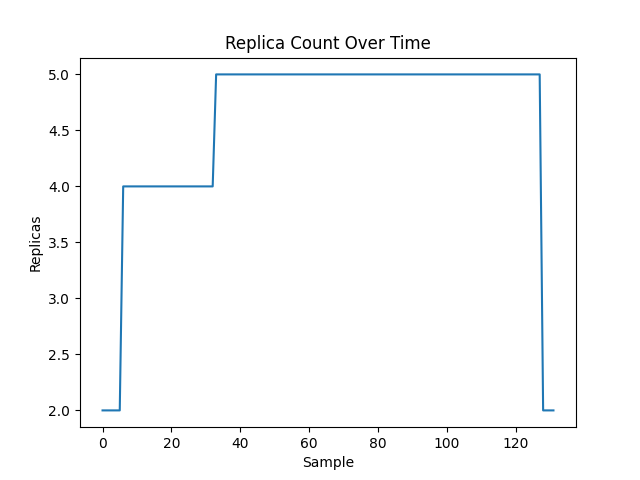
\includegraphics[width=\columnwidth]{figures/experiment-a-hpa/replicas.png}
\caption{Results from Experiment A establishing a correct-behavior baseline.}
\label{fig:exp_a_replicas}
\end{figure}

\noindent\textbf{Takeaway.} HPA does scale correctly when CPU tracks connections
perfectly. The rest of the experiments look at what happens once that
correlation breaks down.

\subsection{Experiment B1: HPA Under Cyclic Load - Over-Provisioning and Recovery
Asymmetry}

\paragraph{Hypothesis.} Under a realistic cyclic HIGH/LOW load pattern - the kind
of thing you'd actually see with real connection activity - HPA should
systematically over-provision and recover slower than it should.

\paragraph{Experimental Setup.} Load alternates between a HIGH phase (800
connections, active CPU-generating pinging, 60~s) and a LOW phase (connections held
open but idle, no pinging, 30~s). During the LOW phase, all 800 client connections
stay open - only the pinging stops, so CPU collapses toward zero while the session
state itself is preserved. \texttt{maxReplicas} was set to 15, and we kept the
default 300-second scale-down stabilization window to see how the factory settings
would perform. We ran five consecutive HIGH/LOW cycles, each 90 seconds.

Results. HPA scaled up to an average peak of 10~replicas. Based on empirical profiling of our server configuration, each pod can sustainably handle approximately 100 active WebSocket connections before CPU utilization reaches the HPA target threshold. During the 60-second ramp-up, the average active connection count was approximately 285, yielding a connection-derived optimum of $\lceil 285/100 \rceil = 3$ replicas. 

The resulting replica over-allocation is computed as:
\begin{equation}
\left( \frac{\text{Observed Replicas (10)}}{\text{Optimal Replicas (3)}} - 1 \right) \times 100 \approx 233\%
\end{equation}

What's driving this is the mismatch between the 90-second cycle and the 300-second window: each
30-second LOW phase ends well before the window has a chance to expire, so every
HIGH phase starts back up near the previous cycle's ceiling. Replicas ratchet up to
10 and just stay there; getting back down to \texttt{minReplicas} after the final
cycle took about 650~seconds. The multi-run average in Figure~\ref{fig:exp_b1_replicas}
confirms this holds across all 3 replications. Variance across replications remained low, indicating consistent behavior.

\begin{figure}[!ht]
\centering
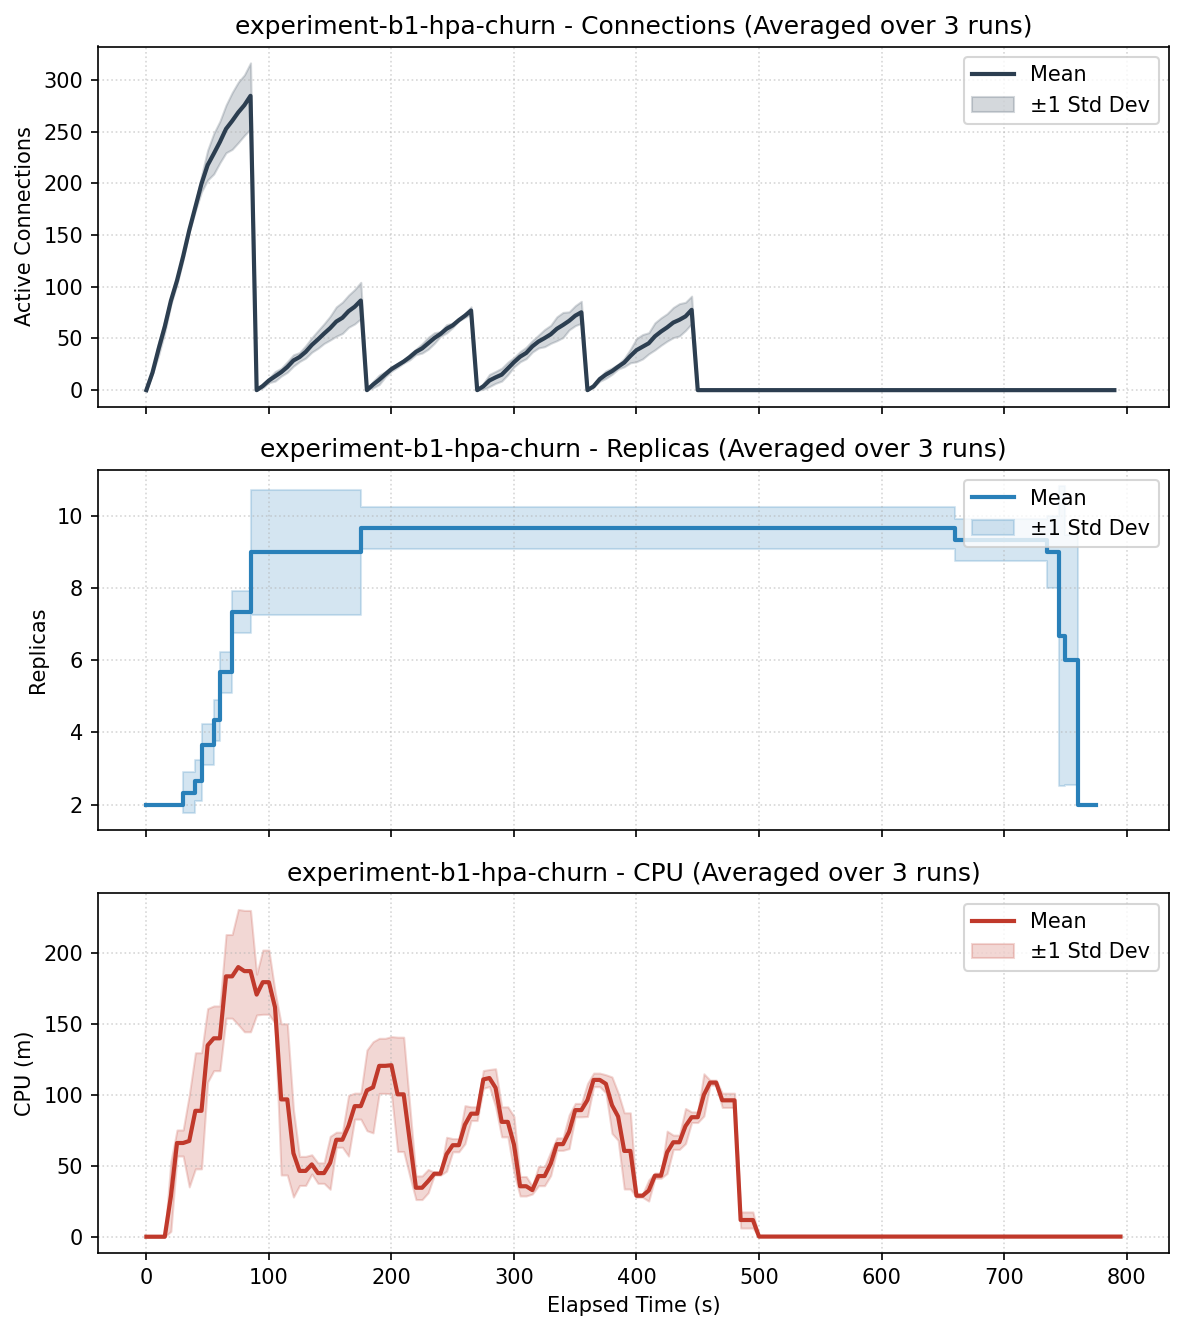
\includegraphics[width=\columnwidth]{figures/experiment-b1-hpa-churn/multi_averaged.png}
\caption{Experiment B1: HPA replica over-allocation under cyclic load.}
\label{fig:exp_b1_replicas}
\end{figure}

Interpretation. HPA simply can't tell the difference between a
LOW period where connections are being held (CPU low, but capacity is still
needed) and one where the pod is genuinely idle. HPA maintained 233\% more replicas than required by the observed connection demand and required approximately 650 seconds to return to the minimum replica count. Although these additional replicas consumed cluster resources, the experiment quantifies replica over-allocation rather than direct infrastructure cost.

\subsection{Experiment B2-Instrumented: Quantifying Reconnection Storm Intensity}

\paragraph{Methodological note.}
Before this, we ran a preliminary, non-instrumented version (B2-Extended LOW) that
confirmed connections were being severed during scale-down, but it gave us no
quantitative data at all - no Prometheus metrics, no storm rate. It was mostly
useful as motivation to add proper instrumentation, and we don't report it as a
standalone result here.

\paragraph{Hypothesis.} Each time HPA scales down and terminates a pod hosting
active connections, we expect a measurable reconnection storm, along with real
instability in the active connection count as clients race to reconnect all at once.

\paragraph{Experimental Setup.} We instrumented the WebSocket server with two
Prometheus metrics: \texttt{active\_connections} (a gauge for the current session
count) and \texttt{new\_connections\_total} (a monotonically increasing counter
that lets us compute rates via \texttt{rate()}). Prometheus scraped at a
15-second interval. HPA was configured with \texttt{stabilizationWindowSeconds: 0}
for scale-up and \texttt{stabilizationWindowSeconds: 60} for scale-down. Setting
scale-up to zero means each reconnection storm - which spikes CPU - immediately
triggers a scale-up, so every cycle produces a complete, observable
scale-up/scale-down sequence within our measurement window. Each cycle was a
60-second HIGH phase (800 pinging clients, \texttt{CPU\_WORK=1}) followed by a
90-second LOW phase (connections idle, no pinging). We picked 90 seconds
specifically because it's longer than the 60-second scale-down window, guaranteeing
HPA executes at least one scale-down per cycle. We ran five complete HIGH/LOW
cycles.

\paragraph{Results.} Every single HPA scale-down event across all five cycles
triggered a distinct, measurable reconnection storm. The storm rates were fairly
consistent run to run, with peak observed rates falling between 406 and
512~conn/s across the replicates. Averaged across the three runs, the mean peak
reconnection rate came out to 457~connections/second (left panel of
Figure~\ref{fig:exp_b2_results}). At the same time, the active connection count got
noticeably unstable during each storm. The mean peak reached 767~($\pm$46), with
individual runs ranging from 732 up to 819 (center panel of
Figure~\ref{fig:exp_b2_results}). That spread - some runs falling below the
800-connection target and others overshooting it - is basically the signature of
a reconnection storm: clients all disconnect at once and race to reconnect,
producing a burst of competing attempts that the server can't resolve
instantaneously.

Here's what's happening at the socket level: once a pod's 30-second termination
grace period ends, it gets \texttt{SIGKILL}, which abruptly resets its TCP
connections (TCP RST). Every client on that pod notices the closure at essentially
the same moment and tries to reconnect right away. That burst of concurrent
\texttt{connect()} calls puts transient pressure on the surviving pods' accept
queues, so some clients end up connecting a little later than others, or fail and
have to retry. That's why the peak connection count can overshoot 800 in one run
(Run~2: 819) and fall short in another (Run~1: 732, Run~3: 750) - it comes down to
exactly when HPA's \texttt{SIGKILL} lands relative to the cycle. The storm itself
settles down within 15-30~seconds once the burst subsides and things stabilize
again.

\begin{figure*}[t!]
\centering
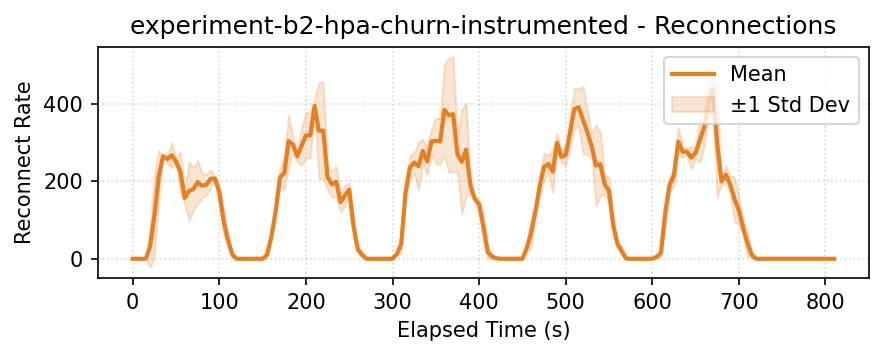
\includegraphics[width=0.32\textwidth]{figures/experiment-b2-hpa-churn-instrumented/multi_averaged_reconnections.png}\hfill
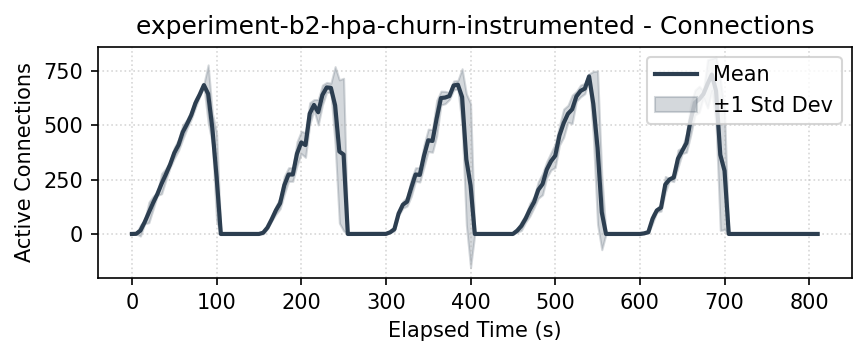
\includegraphics[width=0.32\textwidth]{figures/experiment-b2-hpa-churn-instrumented/multi_averaged_connections.png}\hfill
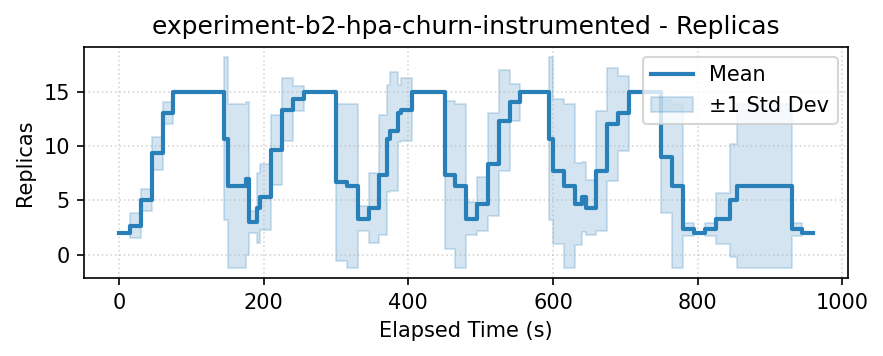
\includegraphics[width=0.32\textwidth]{figures/experiment-b2-hpa-churn-instrumented/multi_averaged_replicas.png}
\caption{Experiment B2-Instrumented: Reconnection storms triggered by HPA scale-down events.}
\label{fig:exp_b2_results}
\end{figure*}

Figure~\ref{fig:exp_b2_results} lays out the replica oscillation and its direct
tie to the client-side session disruption we see in all three metrics.

\noindent\textbf{Observation.} Across the five cycles we measured, every HPA
scale-down event lined up with a measurable reconnection storm. Each time replicas
dropped, all sessions on the terminated pod got disconnected, and the storm's
intensity scaled with how many connections that particular pod was holding. At a
mean peak of 457~conn/s, with the active connection count varying widely across
runs (767~$\pm$46), storms of this size mean a real service disruption for
anything latency-sensitive - the session population just isn't stable or
predictable during the reconnection burst.

\subsection{Experiment B3: Permanent Connection Loss Under Non-Reconnecting Clients}
\label{sec:b3}

\paragraph{Hypothesis.} If WebSocket clients don't implement any reconnection
logic - think batch data collectors, embedded IoT sensors, or long-running
streaming sessions that treat a dropped connection as a terminal failure - then
HPA scale-down events should cause a \textit{permanent, irrecoverable} drop in the
total session population.

\paragraph{Experimental Setup.} We reconfigured the load generator with
\texttt{reconnect: false}, so once a client's connection gets severed by a pod
being terminated, it neither retries nor reconnects. The HPA policy matched
B2-Instrumented: \texttt{stabilizationWindowSeconds: 0} for scale-up,
\texttt{stabilizationWindowSeconds: 60} for scale-down. We kept CPU work on
(\texttt{CPU\_WORK=1}) so HPA would stay active. The IDLE phase ran for up to
240~seconds (\texttt{IDLE\_MAX\_DURATION=240}), giving HPA plenty of room to
execute several sequential scale-down events.

\paragraph{Pod termination mechanics and the 30-second limbo}
It's worth walking through the exact Kubernetes pod termination
sequence~\cite{k8s_pod_lifecycle} here, since it matters for interpreting this
experiment. When HPA reduces \texttt{spec.replicas}, this is what happens, in
order: first, the target pod gets pulled from the Service's endpoint slice
immediately, so no new connections get routed to it. Second, Kubernetes sends
\texttt{SIGTERM} to the pod's main process and starts the
\texttt{terminationGracePeriodSeconds} timer (30~s by default). Third, during that
30-second grace period, the existing TCP connections on the terminating pod stay
open and functional - the OS kernel keeps them alive, not Kubernetes. Fourth, once
\texttt{terminationGracePeriodSeconds} runs out, Kubernetes sends \texttt{SIGKILL},
which kills the process and forces the OS to reset every open TCP connection (TCP
RST). This is why the connection drop in Figure~\ref{fig:exp_b3_results} (left)
lags roughly 30 seconds behind HPA's actual scale-down decision - the connection
doesn't die the instant HPA acts, it dies 30 seconds later when \texttt{SIGKILL}
finally fires. That delay doesn't soften the blow, though: the connection still
dies, the client still gets a TCP RST, and with \texttt{reconnect: false} the
session is gone for good.

\paragraph{Results.} The active connection count (Figure~\ref{fig:exp_b3_results},
left) traces out a clear \textbf{staircase step-down} pattern. Each step lines up
exactly with an HPA scale-down decision - when a pod gets terminated, its entire
connection table is wiped out permanently. Every successive scale-down leaves
fewer active connections than before, with nothing to bring them back. The
representative run (Run~4 of the five-run replication; see
Table~\ref{tab:b3_replication}) went $800 \rightarrow 771 \rightarrow 708
\rightarrow 644$, a 19.5\% permanent loss.

\begin{figure*}[t!]
\centering

\includegraphics[width=0.48\textwidth]{figures/experiment-b3-hpa-idle-connections/connections.png}\hfill

\includegraphics[width=0.48\textwidth]{figures/experiment-b3-hpa-idle-connections/combined.png}
\caption{Experiment B3: Staircase session destruction due to HPA scale-down.}
\label{fig:exp_b3_results}
\end{figure*}

The combined view (Figure~\ref{fig:exp_b3_results}, right) shows how all three
signals relate over time: connections go idle and stop generating CPU load, HPA
sees near-zero CPU and decides to scale down, and the terminated pod then
permanently wipes out every connection it was hosting. None of this can be fixed
just by tweaking a configuration parameter - it follows directly from how HPA
observes, or rather fails to observe, connection state in the first place.

\noindent\textbf{Summary.} Under the configuration we tested, HPA's CPU-based
signal leads it to scale down in ways that destroy idle-but-connected sessions.
Parameter tuning alone doesn't fix this. Recent adaptive threshold approaches improve scaling decisions under varying workloads~\cite{pozdniakova2024sla}; however, they still depend on resource-utilization metrics and therefore do not address connection affinity. This is exactly why future work investigates a connection-aware autoscaling mechanism.

\paragraph{Replication and Statistical Validation}
To make sure this staircase destruction pattern isn't just a one-off artifact, we
replicated Experiment~B3 five times under identical conditions: same Kind cluster
setup, same HPA policy (\texttt{stabilizationWindowSeconds: 60} for scale-down),
800 non-reconnecting clients, and the same two-phase protocol (120-second CONNECT
phase followed by a 240-second IDLE phase). Each run used a freshly provisioned
cluster so there was no state carrying over between replications.
Table~\ref{tab:b3_replication} lays out the per-run connection counts and loss
percentages, and Table~\ref{tab:b3_steps} shows the active connection count at
each observed staircase step for every run.

\begin{table}[!ht]
\centering
\caption{Statistical replication of Experiment B3 (5 runs).}
\label{tab:b3_replication}
\begin{tabular*}{\columnwidth}{@{\extracolsep{\fill}}lccc@{}}
\toprule
\textbf{Run} & \textbf{Peak Conn.} & \textbf{Final Conn.} & \textbf{Loss (\%)} \\
\midrule
Run 1 & 800 & 637 & 20.4\% \\
Run 2 & 800 & 652 & 18.5\% \\
Run 3 & 800 & 658 & 17.8\% \\
Run 4 & 800 & 644 & 19.5\% \\
Run 5 & 800 & 656 & 18.0\% \\
\midrule
\textbf{Mean $\pm$ SD} & \textbf{800 $\pm$ 0} & \textbf{649.4 $\pm$ 8.8} & \textbf{18.8\% $\pm$ 1.1\%} \\
\bottomrule
\end{tabular*}
\end{table}

\begin{table}[!ht]
\centering
\caption{Active connection count at each observed staircase step during the IDLE phase for all five B3 replications.}
\label{tab:b3_steps}
\begin{tabular*}{\columnwidth}{@{\extracolsep{\fill}}lcccc@{}}
\toprule
\textbf{Run} & \textbf{Step 0} & \textbf{Step 1} & \textbf{Step 2} & \textbf{Final} \\
\midrule
Run 1 & 800 & 740 &-& 637 \\
Run 2 & 800 & 718 & 686 & 652 \\
Run 3 & 800 & 761 & 668 & 658 \\
Run 4 & 800 & 771 & 708 & 644 \\
Run 5 & 800 & 741 & 735 & 656 \\
\bottomrule
\end{tabular*}
\end{table}

A few things about these results make us fairly confident the staircase pattern is
a deterministic consequence of how HPA is built, rather than something random:

\begin{enumerate}[leftmargin=*]
\item \textbf{The destruction magnitude barely moves between runs.} Final
connection counts across all five runs sit in a narrow 637-658 band, giving a
standard deviation of just 8.8~connections (1.1\% in loss terms). That kind of low
variance tells us the number of connections lost per scale-down event comes down to
how connections happen to be distributed across pods, not random chance.

\item \textbf{The staircase shape itself never changes.} Every single run goes
through the same three phases: a monotonic climb from 0 to 800 during the CONNECT
phase, a short plateau at 800 while CPU is still elevated, and then a staircase
descent once CPU drops and HPA starts scaling down. How many steps you see (2 or 3)
depends on exactly when HPA's evaluation cycle lines up with the start of the IDLE
phase, but the overall shape doesn't change.

\item \textbf{Loss per step varies, but for a clear reason.} Individual scale-down
steps destroy anywhere from 6 to 163~connections, which just reflects however many
connections the terminated pod happened to be holding. That variation comes from
Kubernetes' round-robin Service routing spreading connections unevenly across
pods, not from any randomness in the HPA control loop itself.
\end{enumerate}

\subsection{Summary Across Experiments}

Table~\ref{tab:failure_summary} pulls together the results from all four
experiments.

\begin{table}[!ht]
\centering
\caption{Summary of results across the four experiments.}
\label{tab:failure_summary}
\resizebox{\columnwidth}{!}{%
\begin{tabular}{@{}p{2.2cm}p{3.5cm}p{3.5cm}p{5cm}@{}}
\toprule
\rowcolor{gray!12}
\textbf{Experiment} & \textbf{Condition} & \textbf{HPA Behavior} & \textbf{Key Quantitative Finding} \\
\midrule
A (Baseline) & Monotonic load; CPU $\propto$ connections & Correct proportional scaling & Works only under idealized signal correlation \\
B1 (Cyclic) & Alternating HIGH/LOW activity & Reaches 10~replicas rapidly & 233\% replica over-allocation; 650~s to recover \\
B2-Inst. (Measured) & Cyclic + Prometheus instrumentation & Reconnection storm per scale-down & Mean peak 457~conn/s; connection instability (767~$\pm$46 peak, range 732--819) \\
B3 (No-reconnect) & Idle connections; no client retry & Permanent, staircase connection loss & $800{\rightarrow}649$ mean final (18.8\% loss); zero recovery \\
\bottomrule
\end{tabular}%
}
\end{table}


%% ============================================================
\section{Discussion}
\label{sec:discussion}
%% ============================================================

\subsection{CPU as a Scaling Signal for Stateful Workloads}
\label{sec:signal_mismatch}

We can capture what's going wrong across Experiments~B1-B3 with two quantities.
Call $M(t)$ the \textit{scaling metric} HPA is watching at time $t$ - under the
standard setup, that's average CPU utilization across all running replicas. Call
$D(t)$ the actual \textit{workload demand} at time $t$: the number of active
connections $C(t)$ whose session state needs to stay alive on a running pod. HPA's
control law (Equation~\ref{eq:hpa}) computes the desired replica count purely from
$M(t)$, and that only gives correct scaling if $M(t)$ actually tracks $D(t)$:
\begin{equation}
M(t) \propto D(t) \quad \Longrightarrow \quad
\textit{desiredReplicas}(t) \propto D(t)
\label{eq:hpa_assumption}
\end{equation}
For stateless HTTP workloads, where each request grabs a bounded chunk of CPU and
lets go of it when it's done, this proportionality basically holds in practice -
Experiment~A backs that up.

For persistent connections that go through idle periods, Equation~\ref{eq:hpa_assumption}
stops holding. While connections are actively pinging, they generate CPU work and
$M(t) \propto D(t)$ still holds. But during idle stretches, the connections are
still open - demand $D(t) = C(t) > 0$ hasn't gone away - while CPU utilization
drops toward zero anyway:
\begin{equation}
M(t) \to 0 \quad \text{while} \quad D(t) = C(t) > 0
\label{eq:websocket_reality}
\end{equation}
Plug that into Equation~\ref{eq:hpa} and \textit{desiredReplicas} gets pushed down
toward \texttt{minReplicas}, so HPA starts scaling down pods that are still hosting
live connections. Put Equations~\ref{eq:hpa_assumption} and
~\ref{eq:websocket_reality} side by side and you get a picture where the scaling
signal and the actual demand move in opposite directions: the metric falls exactly
when demand is at its highest.

What we saw in Experiments~B1, B2-Instrumented, and B3 lines up with this account.
In B3 specifically, CPU utilization fell toward zero because connections had gone
idle, and that drop happened before every scale-down decision. Variance across replications remained low, indicating consistent behavior. Put all three
experiments together and they support the idea that CPU utilization, at least in
the setups we tested, just isn't a reliable stand-in for WebSocket session demand
- and sometimes moves the exact opposite way. Proper metric selection is critical for stability, as demonstrated for containerized applications under varying workloads~\cite{casalicchio2019performance}, and is further complicated by Kubernetes' inherent resource management and scheduling overheads~\cite{medel2024characterising}.

A connection-aware controller explored in subsequent work gives us a useful comparison point: a controller running at
\texttt{CPU\_WORK=0} for 570 seconds holds steady at 8~replicas using nothing but a
connection-count signal. That fits with the idea that the problem here comes down
to which signal HPA is watching, not the proportional control law from Equation~\ref{eq:hpa} itself - give
the same control law a signal that actually tracks $D(t)$, and it does exactly what
you'd expect. Recent intelligent autoscalers improve scaling decisions~\cite{khaleq2023intelligent}, but this does not bypass the fundamental requirement of tracking connection state. Large-scale production deployments have likewise adopted Kubernetes custom metrics infrastructures to improve observability and operational stability~\cite{tedeschi2021cmsweb}. Recent research has focused on jointly optimizing pod- and infrastructure-level elasticity for better resource utilization~\cite{entrialgo2024joint}, whereas our work focuses on preserving application correctness under persistent connection workloads.

\subsection{The Stabilization Window and Idle Connections}

One obvious fix people suggest is just making HPA's stabilization window bigger so
it outlasts the expected idle period. The tuning study in
Section~\ref{sec:tuning_study} shows this doesn't help much, and the reason has
more to do with what the window is actually buffering than with how big it is.

The stabilization window works on a time series of \textit{desiredReplicas}
values, and each one comes from a CPU observation. If CPU stays near zero for the
whole idle period, every value going into that buffer is \texttt{minReplicas}.
Since the stabilized output is just the maximum over the buffer, you end up at
\texttt{minReplicas} no matter how the window is sized - a longer window just
delays the outcome, it doesn't change it.

If instead the window buffered \textit{connection-derived} desired counts - a
rolling high-water mark of recent capacity needs computed straight from the
connection metric - it would be buffering something completely different from
what HPA currently produces. That's a change to what the mechanism operates on,
not just its parameters, which is explored in subsequent work.

\subsection{Pod Termination Timing}

Kubernetes' pod termination sequence leaves a 30-second gap between
\texttt{SIGTERM} and \texttt{SIGKILL} during which connections on the terminating
pod are still open at the OS level. Some people treat this as a chance for
graceful draining via \texttt{preStop} hooks. But WebSocket sessions typically run
for minutes to hours, so a 30-second window is tiny by comparison, and it's not
much use for connection migration or draining in this context.

A better place to intervene might be earlier in the sequence - right where the
scale-down decision itself gets made, before termination even starts. If you
suppress or delay that decision while a pod still has live sessions on it, you fix
the problem at the source rather than trying to patch things during the
termination window. That's the direction we take in subsequent work.

\subsection{HPA Stabilization Window Tuning Study}
\label{sec:tuning_study}

A natural question is whether aggressively tuning
\texttt{scaleDown.stabilizationWindowSeconds} to outlast the expected idle gap
could fix HPA's destructive behavior during idle phases. We tested this directly
with a systematic tuning study across four window sizes - 30, 60, 120, and
300~seconds - each tested under two different gap conditions.

\paragraph{Experimental Methodology.}
For each window size $W \in \{30, 60, 120, 300\}$~seconds, we ran the B3 workload
protocol (800 non-reconnecting clients, 120-second CONNECT phase with
\texttt{CPU\_WORK=1}) followed by an idle gap of length $G$. We tested two
conditions per window: $G < W$ (``below,'' where the gap is shorter than the
window and connections should be protected), and $G > W$ (``above,'' where the gap
outlasts the window and HPA is expected to scale down). We picked
$G_{\text{below}} = W - 15$~s and $G_{\text{above}} = W \times 1.5$ to $W + 60$~s,
giving margin on both sides of the boundary. All eight configurations (4 windows
$\times$ 2 gap conditions) were replicated three times each on fresh Kind
clusters, for 24~sub-experiments in total.

\paragraph{Results.}
Table~\ref{tab:tuning_results} shows the aggregated results. The pattern couldn't
be clearer: when the idle gap sits below the stabilization window, connections
survive every time (0\% loss across all 12~below-window runs). Once the gap
exceeds the window, connections get destroyed in every configuration we tested,
with mean loss rates running from 5.2\% at a 30-second window up to 33.2\% at a
300-second window.

\begin{table}[!ht]
\centering
\caption{HPA stabilization window tuning study results (3 replications per configuration).}
\label{tab:tuning_results}
\begin{tabular*}{\columnwidth}{@{\extracolsep{\fill}}cccrr@{}}
\toprule
\textbf{Window} & \textbf{Gap} & \textbf{Relation} & \textbf{Loss (\%)} & \textbf{Survived} \\
\midrule
30s  & 15s  & below & $0.0 \pm 0.0$ & 3/3 \\
30s  & 90s  & above & $5.2 \pm 6.2$ & 2/3 \\
\midrule
60s  & 45s  & below & $0.0 \pm 0.0$ & 3/3 \\
60s  & 120s & above & $10.2 \pm 7.2$ & 2/3 \\
\midrule
120s & 105s & below & $0.0 \pm 0.3$ & 3/3 \\
120s & 180s & above & $10.4 \pm 5.6$ & 1/3 \\
\midrule
300s & 285s & below & $0.0 \pm 0.0$ & 3/3 \\
300s & 360s & above & $33.2 \pm 28.0$ & 1/3 \\
\bottomrule
\end{tabular*}
\end{table}

\begin{figure}[!ht]
\centering
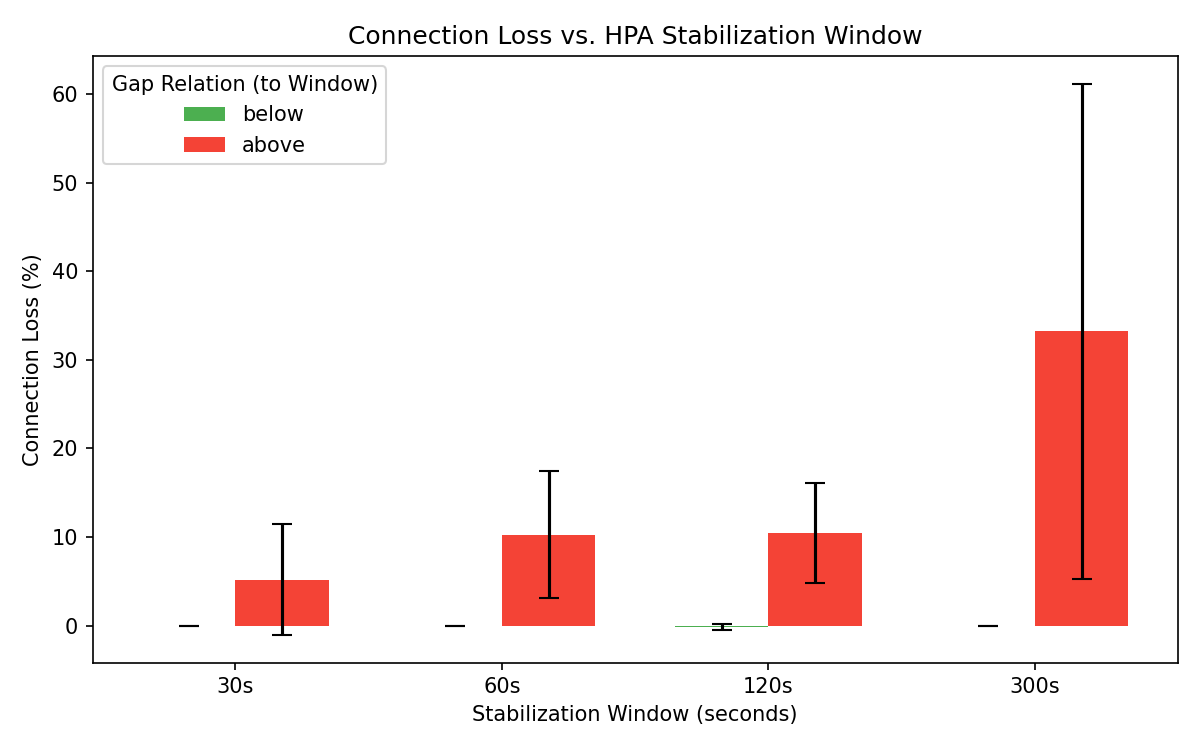
\includegraphics[width=\columnwidth]{figures/tuning_results_loss.png}
\caption{Connection loss percentage relative to the HPA stabilization window and gap duration.}
\label{fig:tuning_results}
\end{figure}

\paragraph{Analysis.}
These results tell us two things about HPA's stabilization mechanism. First, the
window works more like a delay than a protection: it pushes the scale-down
decision back by $W$~seconds without ever actually preventing it. If CPU stays
near zero for the whole window, every entry in the recommendation buffer converges
to \texttt{minReplicas}, and the stabilized output - the max over the window -
ends up at \texttt{minReplicas} too.

Second, the variance in the ``above'' condition gets a lot bigger at larger window
sizes (SD~$= 28.0\%$ at $W=300$s versus SD~$= 6.2\%$ at $W=30$s), which is probably
tied to how HPA's 15-second evaluation cycle lines up with the window boundary.
When the idle gap only barely exceeds the window, whether a scale-down event
actually lands inside the measurement period depends on that alignment - which
adds variance that has nothing to do with the window's protective effect.

Across every window size we tested, we never found a configuration where a finite
stabilization window actually prevented connection loss once the idle gap outlasted
the window. That fits with the idea that the window is a buffer on CPU-derived
recommendations, not a mechanism that's actually sensitive to connection state.

%% ============================================================
\section{Threats to Validity and Limitations}
\label{sec:limitations}
%% ============================================================

\begin{enumerate}[leftmargin=*]

\item \textbf{Evaluation environment.} We ran every experiment on a single-machine
Kind cluster. That gives us full reproducibility and tight control, but it doesn't
capture cross-node scheduling latency, network partitions, or the metric-collection
noise you'd see on a real multi-node cloud cluster. The direction of our results
should hold up; the exact timing numbers (pod startup lag, HPA sync precision) may
look different on production infrastructure. Although our experiments were conducted on a Kind cluster, similar Kubernetes monitoring architectures have been deployed successfully in large-scale production environments such as CERN CMSWEB~\cite{tedeschi2021cmsweb, ali2024cmsweb}. Validation of these dynamics on managed Kubernetes offerings (such as GKE, EKS, or AKS) is left for future work.

\item \textbf{Workload generalizability.} Our load generator uses a synthetic
WebSocket workload with a linear connection ramp and deterministic silence gaps.
Real-world connection arrival tends to be burstier, and session durations vary a
lot more. Under stationary random load (Poisson arrivals), we'd expect the same
proportional failure mechanisms to apply; only the peak connection count and storm
rate we observed would likely change.

\item \textbf{Instrumentation dependency.} The B2-Instrumented results depend on
Prometheus scraping metrics every 15 seconds. A coarser scrape interval would
affect how precisely we can measure the storm rate, but it wouldn't change the
underlying causal finding that scale-down events trigger reconnection cascades.

\item \textbf{Protocol generalizability.} The evaluation focuses on CPU-based HPA and WebSocket workloads. Other stateful protocols such as MQTT or gRPC streaming may exhibit different quantitative behavior although similar qualitative limitations are expected.

\item \textbf{Single reconnect=false regime.} Experiment~B3 uses a uniform
\texttt{reconnect: false} policy across the board. Real deployments usually have a
mix of reconnecting and non-reconnecting clients, so the staircase destruction rate
and the final session population would likely look different under a mixed
client policy.

\end{enumerate}



%% ============================================================
\section{Conclusion}
\label{sec:conclusion}
%% ============================================================

This paper looked at how Kubernetes HPA behaves under stateful WebSocket workloads
through four controlled experiments, each one building on the last.

Experiment~A showed HPA scales correctly when CPU tracks connections perfectly -
a condition that's rarely true outside a lab. Experiment~B1 put HPA through a
realistic HIGH/LOW activity cycle and produced 233\% replica over-allocation (10 replicas
instead of the correct 3), hit \texttt{maxReplicas} within 99~seconds, and took
roughly 650~seconds to recover. Experiment~B2-Instrumented added Prometheus
instrumentation and directly measured what scale-down actually costs: a peak
reconnection rate of 457~connections/second, and real instability in the active
connection count (mean peak of 767~$\pm$46, ranging from 732 to 819 against an
800-client target), both lining up exactly with HPA's scale-down events.
Experiment~B3, with reconnection turned off, produced a staircase pattern of
permanent connection loss - across five replications, the session population
dropped from 800 to a mean of 649 ($\pm$1.1\%, or 18.8\% loss), with nothing
bringing it back.

Put together, these results point to a limitation that has more to do with how HPA
is designed than with any one configuration choice. CPU utilization, at least in
the setups we tested, doesn't work as a reliable stand-in for connection-based
demand, and the tuning study in Section~\ref{sec:tuning_study} shows that adjusting
the stabilization window doesn't really change that once the idle period outlasts
the window. The window buffers CPU-derived recommendations, not connection counts
- the problem is what gets measured, not how long the measurement gets held onto.

One takeaway from all this is that autoscaling for stateful, persistent-connection
workloads probably needs two things working together: a scaling signal built
directly from connection counts, since that reflects session state honestly, and
scale-down logic that actually checks for live sessions before it terminates a pod.
These findings give future connection-aware autoscaling work a quantitative
baseline to build on, and they make a decent case for rethinking CPU-centric
autoscaling wherever persistent, cloud-native applications are involved.



\section*{Declarations}

\begin{itemize}
\item \textbf{Data Availability} The source code, Kubernetes manifests, Prometheus dashboards, experimental scripts, datasets, and plotting utilities used in this study are publicly available at: \url{https://github.com/MistaHolmes/ws-k8-controller}.
\item \textbf{AI Declaration} During the preparation of this manuscript, the authors used generative AI tools, including Claude and ChatGPT, to assist with language refinement, grammar correction, manuscript organization, and editorial improvements. The study conception, methodology, software implementation, experimental design, data collection, analysis, interpretation of results, and scientific conclusions were developed, verified, and approved by the authors. The authors carefully reviewed and edited all AI-assisted content and take full responsibility for the final manuscript.
\end{itemize}

%% ============================================================
\bibliographystyle{spmpsci}
\bibliography{reference}

\end{document}